\section{Memory Layout}
\label{sec:enclaves}

The central context of SGX is the \textit{enclave}, a protected environment
that contains the code and data pertaining to a security-sensitive computation.
This section provides an overview of the data structures used by an enclave.


\subsection{Memory Ownership vs Management}

% Access Control Requirements: SGX S 2.3

Enclaves use RAM to store their code and data, and need logical processors to
execute their code in order to perform the computation they were designed to
do. These computer resources are traditionally managed by privileged software,
such as hypervisors and operating system kernels.

In order for SGX to fit into this design, the code inside SGX enclaves is
subjected to the same address translation mechanism (\S~\ref{sec:paging}) as
the applications that enclose the enclaves. Enclave code runs at ring 3
(\S~\ref{sec:rings}), just like application code, so that it cannot
interfere with the privileged software that manages resources.

% Interactions with VMX: SGX S 6.5, 6.5.{1,2,3,4,5}

The rest of the paper will use the term \textit{system software} to refer to
the privileged software that manages resources. On most computers, this is an
operating system kernel. When VMX is in use, SGX resources are allocated by
the hypervisor to guest operating systems running in virtual machines.


\subsection{Enclaves in RAM}

% PRM: SGX S 3.5

The enclaves' code and data is stored in \textit{Processor Reserved Memory}
(PRM), a contiguous range of RAM that cannot be directly accessed by other
software, including privileged software such as the SMM code, the hypervisor,
and the OS kernel. The memory controller is integrated on the CPU die (see
Figure~\ref{fig:cpu_die}), so it can be trusted to prevent devices attached to
the system bus from performing DMA transfers to/from the PRM.

Rejecting improper accesses to PRM is central to the SGX security model. The
designers were aware of that, and took clear steps to reduce the complexity of
the PRM checks, which in turn reduces the probability of bugs in the
implementation. The PRM must be set up to use SGX features and, once
configured, the PRM range cannot be changed. Furthermore, the PRM's size must
be an integer power of two, and its start address must be aligned to the same
power of two. The range restrictions reduce the complexity of checking if a RAM
address is in the PRM to a bitwise AND and an equality comparison.

\begin{figure}[hbt]
  \center{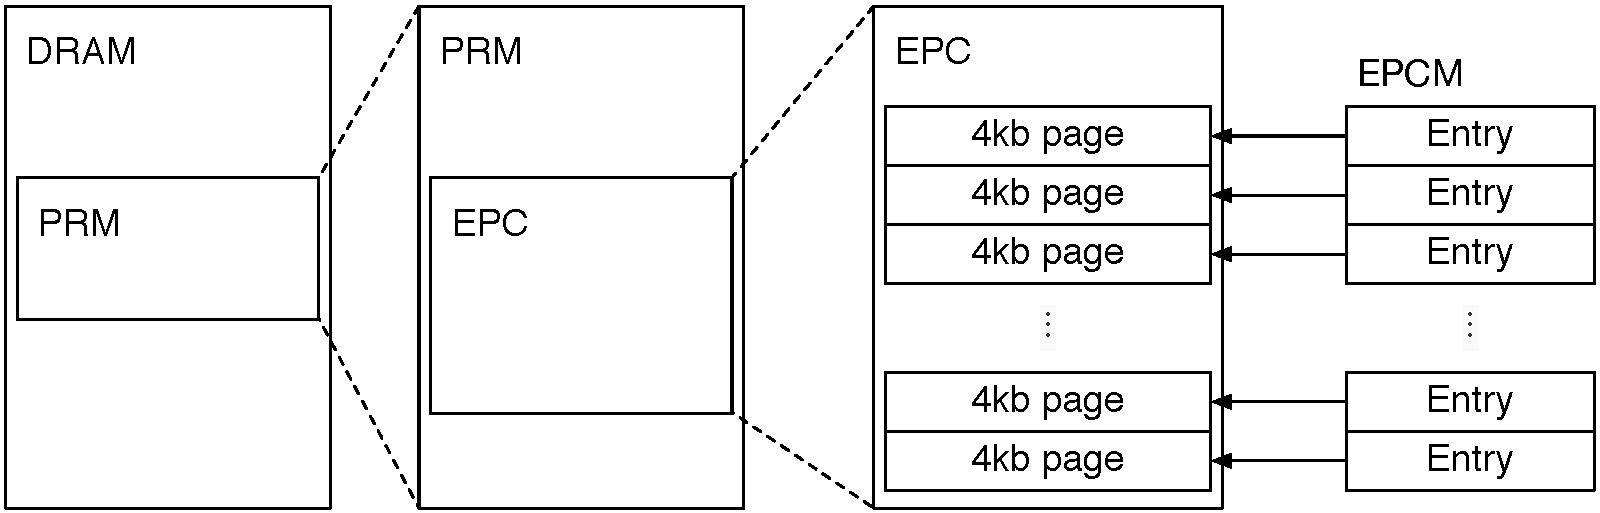
\includegraphics[width=85mm]{figures/sgx_epc.pdf}}
  \caption{
    Enclave data is stored into the EPC, which is a subset of the PRM. The
    PRM is a contiguous range of RAM that cannot be accessed by system software
    or peripherals.
  }
  \label{fig:sgx_epc}
\end{figure}


\subsection{The Enclave Page Cache (EPC)}

% EPC and EPCM: SGX S 1.5, S 1.5.1, S 2.6.13, S 3.5, S 3.5.1

The contents of enclaves and the associated data structures are stored in the
\textit{Enclave Page Cache} (EPC), which is a subset of the PRM.

The SGX design handles multiple enclaves active at the same time, which is
necesssary in multi-tasking environments. This is achieved by having the EPC
split into 4kb pages, which can be associated to different enclaves. The system
software is responsible for allocating physical EPC pages to enclaves, using
specific SGX instructions.

The CPU maintains some metadata for each EPC page into the \textit{Enclave Page
Cache Map} (EPCM). The metadata tracks the enclave that each page was allocated
to, so the processor can prevent the code inside an enclave from accessing EPC
pages that belong to other enclaves.

The EPCM metadata for a page also includes the expected linear address used to
access the page. When an EPC page is accessed, the processor che

% types
access another enclave's pages, and that system software manages EPC pages in a
way that is consistent with the SGX security model.


The SGX documentation does
not state where the EPCM is stored, but we can hypothesize that it is either
an on-chip memory, like the L3 cache, or stored in a PRM region that is not
used by the EPC.


% EPCM table: SGX S 2.6.13

\begin{table}[hbt]
  \center{\begin{tabularx}{\columnwidth}{| l | r | X |}
  \hline
  \textbf{Field} & \textbf{Bits} & \textbf{Description}\\
  \hline
  VALID & 1 & 0 for un-allocated EPC pages \\
  \hline
  BLOCKED & 1 & page is being evicted (\S~\ref{TBD})\\
  \hline
  R & 1 & allow reads by enclave code\\
  \hline
  W & 1 & allow writes by enclave code\\
  \hline
  X & 1 & allow execution of code inside the page, inside enclave\\
  \hline
  EID & 64 & the ID of the enclave that owns the page\\
  \hline
  PT & 8 & the page type (SECS, TCS, VA, regular)\\
  \hline
  LINADDR & 48 & the \\
  \hline
  \end{tabularx}}
  \caption{
    The fields in an EPCM entry.
  }
  \label{fig:epcm_entry}
\end{table}


% SECINFO: SGX S 2.6.5, S 2.6.5.{1,2}


\subsection{Enclave Identity}

% Main data structures: SGX S 1.4
% SECS: SGX S 2.6.1, S 2.6.1.1, S 3.1
% ECREATE: SGX S 3.1, S 5.3
% Implicit access: SGX S 2.3

The first step in creating an enclave is using the \texttt{ECREATE} instruction
to designate an EPC page that becomes the enclave's \textit{SGX Enclave Control
Structure} (SECS). All other instructions that operate on an enclave access the
enclave's SECS directly or indirectly.

Once created, the SECS page is not directly accessible by enclave code, and its
exact format is not specified in the SGX documentation. \texttt{ECREATE} does
read a 4kb page from non-EPC memory, the contents of which is used to specify
a number of enclave properties.

The SECS has two fields (BASEADDR and SIZE) that specify the enclave's linear
address space (ELRANGE in the Intel documentation). The enclave's starting
address has to be aligned by the enclave size, which simplifies checking if a
linear address belongs to an enclave or not, just like in the case of PRM
physical addresses.

The SECS also specifies the Intel architecture features used by the enclave
code, in the ATTRIBUTES field. This

\texttt{ECREATE} generates a 64-bit enclave ID (EID) that is stored at an
unspecified location inside the SECS. The EID is used to identify the enclave's
pages in the EPCM.



The SGX documentation does not reveal the exact layout of the SECS page in the
EPC.  \texttt{ECREATE}





% TCS: SGX S 2.6.2, S 2.6.2.{1,2,3,4}


% SSA: SGX S 2.6.3,
